% BUET CSE 450 Capstone Project Report
\documentclass[12pt,a4paper,oneside]{report}
\usepackage{cse-capstone}

\newcommand{\ProjectTitle}{Leveraging Temporal Information for Robust Liveness Verification}
\newcommand{\Session}{\TBC{Session}}
\newcommand{\SubmissionDate}{\TBC{Submission month and year}}
\newcommand{\Supervisors}{\TBC{Supervisor name and designation}\\Department of CSE, BUET}

\hypersetup{
  pdftitle={\ProjectTitle},
  pdfauthor={Nafis Nahian; Abrar Zahin Raihan; Aritra Debnath; Tamzeed Mahfuz; Ruwad Naswan},
  pdfsubject={CSE 450 Capstone Project Report},
  pdfkeywords={face liveness, deepfake detection, temporal modelling, domain generalisation, specialist routing}
}

\begin{document}

\pagenumbering{gobble}
\thispagestyle{empty}
\begin{center}

{\large CSE 450 Capstone Project Report}

\vspace*{\stretch{2}}
{\LARGE\bfseries \ProjectTitle}

\vspace*{\stretch{4}}
{\large Submitted by}\\[10pt]
\begin{tabular}{ll}
  Nafis Nahian & 2105007 \\
  Abrar Zahin Raihan & 2105009 \\
  Aritra Debnath & 2105010 \\
  Tamzeed Mahfuz & 2105012 \\
  Ruwad Naswan & 2105051
\end{tabular}

\vspace*{\stretch{3}}
{\large Supervised by}\\[10pt]
\Supervisors

\vspace*{\stretch{3}}

\includegraphics[width=30mm]{buet_logo.png}\\[8pt]
\textbf{Department of Computer Science and Engineering}\\
{\large\bfseries Bangladesh University of Engineering and Technology}\\
Dhaka, Bangladesh

\vspace*{\stretch{1}}
\Session\\
\SubmissionDate

\end{center}
\clearpage


\pagenumbering{roman}
\chapter*{Candidates' Declaration}
\addcontentsline{toc}{chapter}{Candidates' Declaration}

We declare that this report presents our own capstone work except where sources,
datasets, pretrained models, software, or ideas are explicitly acknowledged. To
the best of our knowledge, it has not been submitted in the same form for another
degree or award. Each candidate accepts responsibility for the integrity of the
reported methods, results, and limitations.

Public research implementations and datasets used by the project are identified
in the report and bibliography. Generative-AI tools were used to assist with
drafting and editing parts of the report; the candidates remain responsible for
checking every technical claim, citation, and numerical result against primary
evidence and for complying with the course's disclosure policy.

\draftnote{Replace or amend the AI-assistance statement if the department or
supervisor prescribes exact disclosure language. Add signatures and dates in the
final signed copy.}

\vspace{18mm}
\begin{tabularx}{\textwidth}{@{}Y Y@{}}
\rule{55mm}{0.4pt} & \rule{55mm}{0.4pt}\\[-1mm]
Nafis Nahian (2105007) & Abrar Zahin Raihan (2105009)\\[14mm]
\rule{55mm}{0.4pt} & \rule{55mm}{0.4pt}\\[-1mm]
Aritra Debnath (2105010) & Tamzeed Mahfuz (2105012)\\[14mm]
\rule{55mm}{0.4pt} & \\
Ruwad Naswan (2105051) &
\end{tabularx}

\clearpage


\chapter*{Acknowledgement}
\addcontentsline{toc}{chapter}{Acknowledgement}

We express our deepest gratitude to our supervisor, \TBC{supervisor name}, for
shaping the research direction, questioning our assumptions, and guiding the
project through its successive temporal, domain-generalisation, and deepfake
detection experiments. In particular, the idea of selecting manipulation-specific
experts through a learned routing model originated from our supervisor. That idea
led to one of the strongest later experimental results and materially improved
our understanding of heterogeneous deepfake attacks.

We thank Pathao for presenting the original financial liveness-verification
problem and for the early project context. The subsequent research and
implementation were carried out independently using public datasets and our own
computing resources; no private Pathao dataset, project grant, or sustained
technical collaboration was received.

We also acknowledge the authors and maintainers of the public datasets, research
implementations, and open-source libraries on which the experiments depended.
Finally, we thank our teachers, classmates, friends, and families for their
feedback and support throughout the capstone.

\clearpage


\chapter*{Abstract}
\addcontentsline{toc}{chapter}{Abstract}

Remote financial identity verification must distinguish genuine users from both
physical presentation attacks and digitally manipulated or injected face media.
This project investigates a layered liveness-verification architecture whose
first stage is a lightweight temporal MobileNetV3 model for mobile inference and
whose stronger experimental components include G2V2Former temporal reasoning,
GD-FAS domain-generalised spatial features, Xception deepfake detectors, and a
learned manipulation-specific routing strategy. The mobile prototype captures a
short clip, samples 24 frames, performs local inference, and applies a fixed
decision threshold. Server escalation, score fusion, capture attestation, and
human review are target-architecture elements rather than completed integrations.

Cross-domain experiments reveal the central difficulty. Under the repository's
common evaluation protocol, GD-FAS trained on LCC-FASD achieved 4.55\% HTER and
99.69\% AUC on LCC-FASD but 52.99\% HTER and 50.49\% AUC on Celeb-DF-v2.
Fine-tuning on Celeb-DF-v2 improved its target-domain result to 41.04\% HTER and
64.35\% AUC while reducing source-domain performance. G2V2Former showed the same
generalisation challenge. A later FaceForensics++ experiment compared a universal
Xception detector with manipulation-specific experts selected by a learned
router. The current six-way routing artefact improved balanced accuracy from
76.44\% to 84.51\% and ROC-AUC from 86.32\% to 91.68\% on a group-disjoint,
in-domain validation split. However, it includes an ``original'' routing class;
therefore it does not yet implement the intended formulation in which a router
estimates the most suitable one of five binary specialists from an embedding.

The work contributes an evidence-based analysis of temporal information,
cross-domain transfer, mobile deployment constraints, and specialist routing. It
also identifies the safeguards required before financial use: capture-channel
integrity, subgroup and cross-domain evaluation, privacy protection, calibrated
thresholds, accessible appeal, and accountable human oversight.

\textbf{Keywords:} face liveness; deepfake detection; temporal modelling; domain
generalisation; specialist routing; mobile inference.

\clearpage


\tableofcontents
\listoffigures
\listoftables

\clearpage
\pagenumbering{arabic}
\chapter{Problem Identification and Formulation}
\label{ch:problem}

\section{Background and Motivation}

Remote onboarding and account recovery frequently compare a selfie or short face
video with identity evidence. The comparison is useful only if the media came
from the person and capture session being verified. An attacker may instead
present a printed photograph, replay a video on another screen, wear a mask,
display a manipulated video, or bypass the physical camera and inject forged
media. ENISA consequently separates camera presentation from injection attacks
and recommends layered controls spanning the client and server
\cite{enisa2022,enisa2024}. NIST likewise treats sensor authenticity, protected
channels, presentation-attack detection (PAD), and forged-media analysis as
complementary controls rather than substitutes \cite{nist80063a4}.

This problem is especially consequential in financial verification. A false
acceptance can enable impersonation and monetary loss, while a false rejection
can exclude a legitimate customer or repeatedly expose their biometric data.
The system must therefore balance security, usability, latency, resource use,
privacy, and equitable performance instead of optimising only dataset accuracy.

Deepfake attacks are difficult for several connected reasons:

\begin{itemize}
  \item manipulation mechanisms are heterogeneous and continue to evolve;
  \item compression, resizing, recapture, and post-processing can erase the
        artefacts on which a detector relies;
  \item a model can learn dataset, identity, background, or codec shortcuts and
        then fail under a new generator or population;
  \item a manipulated face can preserve plausible blinking, pose, and motion, so
        conventional liveness cues alone do not establish authenticity;
  \item a virtual camera or compromised client can bypass assumptions about a
        trusted physical capture path; and
  \item mobile inference restricts model size, memory, energy, and response time.
\end{itemize}

The attack must consequently be described along more than one axis.
\Cref{fig:taxonomy} distinguishes the delivery path from the manipulation family.
The five FaceForensics++-derived experimental fake classes are not five equivalent
meanings of ``deepfake'': Deepfakes, FaceSwap, and FaceShifter are identity-swap
approaches, whereas Face2Face and NeuralTextures are reenactment/neural-rendering
approaches \cite{rossler2019faceforensics,li2020faceshifter}. ``Original'' denotes
genuine data and is not a manipulation class.

\begin{figure}[H]
  \centering
  \begin{tikzpicture}[
  font=\small,
  box/.style={draw=buetblue,rounded corners,fill=softblue,align=center,minimum height=11mm,text width=37mm},
  leaf/.style={draw=gray!75,rounded corners,fill=white,align=center,minimum height=10mm,text width=37mm},
  arr/.style={-{Latex[length=2.2mm]},thick,draw=buetblue}
]
\node[box] (capture) {Delivery path};
\node[leaf,below left=12mm and 17mm of capture] (physical) {Physical presentation\\print, replay, mask};
\node[leaf,below=12mm of capture] (recapture) {Deepfake recaptured\\through a display};
\node[leaf,below right=12mm and 17mm of capture] (inject) {Digital injection\\virtual camera or API};
\draw[arr] (capture) -- (physical);
\draw[arr] (capture) -- (recapture);
\draw[arr] (capture) -- (inject);

\node[box,below=23mm of recapture] (family) {Manipulation family};
\node[leaf,below left=12mm and 17mm of family] (swap) {Identity swap\\Deepfakes, FaceSwap,\\FaceShifter};
\node[leaf,below=12mm of family] (reenact) {Reenactment\\Face2Face,\\NeuralTextures};
\node[leaf,below right=12mm and 17mm of family] (outside) {Outside experiment\\full synthesis, lip-sync,\\audio or document fake};
\draw[arr] (family) -- (swap);
\draw[arr] (family) -- (reenact);
\draw[arr] (family) -- (outside);
\end{tikzpicture}


  \caption{Threat taxonomy used in this report. Delivery path and manipulation
  family are separate: the same generated video may be shown to a camera or
  injected directly. Items outside the experiment remain relevant threats.}
  \label{fig:taxonomy}
\end{figure}

\section{Problem Statement}

The engineering problem is to design and evaluate a practical face-liveness
screening pipeline for remote financial verification that detects both physical
presentation attacks and digitally manipulated faces, uses temporal evidence
where useful, degrades safely under uncertainty, and remains feasible on a
mobile--server architecture. The work asks four linked questions:

\begin{enumerate}
  \item Can a lightweight temporal model provide a useful first decision on a
        mobile device?
  \item How well do stronger temporal and domain-generalised PAD models transfer
        from physical-spoof datasets to deepfake datasets?
  \item Does manipulation-specific expertise improve frame-level deepfake
        detection relative to one universal detector?
  \item What security and ethical controls are required before experimental
        accuracy can become a trustworthy financial decision?
\end{enumerate}

For a captured clip $V=(x_1,\ldots,x_K)$, the first-layer model produces a fake
probability $p_1=p(\mathrm{fake}\mid V)$. A target cascade uses two policy
thresholds $\tau_{\mathrm{pass}}<\tau_{\mathrm{attack}}$: clear low-risk cases
may pass, clear high-risk cases may be rejected or challenged, and the interval
between them is escalated. These thresholds are a design requirement; the current
Flutter prototype applies a single threshold of 0.5.

For the later specialist experiment, let $x$ be a preprocessed face frame,
$z=\phi(x)$ an embedding, and $\mathcal{E}$ the five manipulation-specific binary
experts. The intended router is

\begin{align}
q_e(z) &= P(E^*=e\mid z), \qquad e\in\mathcal{E},\\
\hat e &= \arg\max_{e\in\mathcal{E}} q_e(z),\\
\widehat p(\mathrm{fake}\mid x) &= s_{\hat e}(x),
\end{align}

where $s_e$ is the fake probability from expert $e$. The router does not predict
``original''; every frame is assigned to a binary specialist. A truthful claim of
$P(\text{best expert}\mid z)$ additionally requires leakage-safe targets---for
example, choosing the expert with the lowest out-of-fold loss for each training
sample under a declared tie rule. If the training target is merely the known
manipulation label, the correct interpretation is
$P(\text{manipulation method}\mid z)$, not the best expert. The current notebooks
use a six-way original-plus-method classifier and an original-route fallback.
They are therefore reported as a legacy six-way routing result and not as a
completed implementation of the intended equations.

\section{Complexity of the Problem}

The project qualifies as a complex engineering problem because its requirements
conflict and its operating conditions are only partially observable. Important
dimensions are summarised in \Cref{tab:complexity}.

\begin{table}[H]
\centering
\caption{Sources of engineering complexity.}
\label{tab:complexity}
\begin{tabularx}{\textwidth}{@{}p{32mm}Y Y@{}}
\toprule
Dimension & Conflict or uncertainty & Engineering implication \\
\midrule
Attack diversity & Prints, replay, reenactment, face swap, recapture, and
injection expose different signals. & No single benchmark or cue demonstrates
complete protection. \\
Domain shift & Dataset, camera, subject, codec, and generator differ from the
deployment domain. & Group-disjoint and cross-domain evaluation are mandatory. \\
Edge constraints & Larger temporal models may improve evidence but increase
latency, memory, energy, and network use. & Use a lightweight local stage and
selective escalation. \\
Decision cost & False accepts create fraud risk; false rejects create exclusion
and support cost. & Calibrate thresholds against operational costs and provide
retry/appeal paths. \\
Biometric sensitivity & Face data is difficult to revoke and may reveal identity
or demographic attributes. & Minimise collection, secure transit and storage,
and define retention and access controls. \\
Adversarial evolution & Attackers can adapt after learning detector behaviour. &
Monitor drift, limit disclosure of exploitable details, and retest continuously. \\
\bottomrule
\end{tabularx}
\end{table}

\section{Project Objectives and Scope}

The project objectives are to:

\begin{enumerate}
  \item establish a clear physical-presentation, manipulation, and injection
        threat model for remote face verification;
  \item build a lightweight temporal first-stage classifier and integrate its
        exported model into a Flutter capture flow;
  \item investigate richer temporal evidence through $G^2V^2$former;
  \item compare temporal modelling with the GD-FAS domain-generalisation method;
  \item measure within-domain and cross-domain behaviour on public PAD and
        deepfake datasets;
  \item compare a universal Xception detector with manipulation specialists and
        learned routing;
  \item specify a layered escalation architecture and the controls needed for
        trustworthy deployment; and
  \item analyse privacy, fairness, accessibility, accountability, intellectual
        property, cost, and environmental impact.
\end{enumerate}

The implemented scope comprises public-data experiments, preprocessing and
training notebooks, a Flutter/mobile temporal prototype, a separately demonstrated
$G^2V^2$former API, GD-FAS evaluation, and frame-level Xception routing experiments.
It does not comprise a production Pathao Pay deployment, a connected multi-model
backend, capture-device attestation, a reviewer console, calibrated production
thresholds, or a completed field trial. Audio deepfakes, document forgery, fully
synthetic identities, and end-to-end identity matching are threat context but not
separately evaluated model classes.


\chapter{Preliminary Research}
\label{ch:research}

\section{Literature Review}

\subsection{Presentation attacks, deepfakes, and injection}

PAD traditionally evaluates whether a biometric sample is bona fide or a
presentation attack at the capture device. ISO/IEC 30107-3 defines principles for
testing and reporting PAD performance, including attack-type classification, but
explicitly excludes attacks outside the capture device from its scope
\cite{iso30107}. This boundary matters: a detector that recognises screen moir\'e
or print texture does not establish that a video stream came from a genuine
camera. ENISA's later guidance therefore treats injection attack detection (IAD)
alongside PAD and recommends a multi-layer client--server approach
\cite{enisa2024}. NIST SP 800-63A-4 similarly calls for confidence in the genuine
sensor, protected communications, manipulated-media analysis, and documented
manual processes \cite{nist80063a4}.

FaceForensics++ provides a controlled benchmark with several facial manipulation
methods and compression levels, and established Xception as a strong baseline
\cite{rossler2019faceforensics,chollet2017xception}. Celeb-DF-v2 was designed with
higher-quality face swaps and fewer conspicuous synthesis artefacts, making it a
more challenging test of shortcut-dependent detectors \cite{li2020celebdf}.
Cross-dataset deepfake work repeatedly shows that strong in-domain performance
does not guarantee unseen-generator performance; video-oriented approaches such
as AltFreezing were developed specifically to improve this transfer
\cite{wang2023altfreezing}.

\subsection{Temporal and domain-generalised face anti-spoofing}

MobileNetV3 uses hardware-aware architecture search and efficient blocks intended
for resource-constrained inference \cite{howard2019mobilenetv3}. In this project,
its per-frame features are averaged over a short clip, providing a simple temporal
baseline without the cost of full spatiotemporal attention.

$G^2V^2$former combines cropped face appearance with facial landmarks. It
factorises spatial and temporal attention, introduces Kronecker temporal
attention, and uses landmark motion to guide facial-expression features
\cite{yang2024g2v2}. It is therefore relevant when motion contains evidence that
is weak or ambiguous in any individual frame.

GD-FAS addresses a different failure mode. Its group-wise scaling risk
minimisation and feature orthogonal decomposition aim to align both the direction
and bias of local decision boundaries while separating domain-invariant from
domain-specific features \cite{jung2025gdfas}. It remains a frame-level spatial
model in this project; comparing it with $G^2V^2$former helps separate the value
of temporal structure from the value of domain-generalised representation.

\begin{table}[H]
\centering
\caption{Research approaches and their roles in the project.}
\label{tab:literature-map}
\begin{tabularx}{\textwidth}{@{}p{28mm}p{27mm}Y Y@{}}
\toprule
Approach & Primary evidence & Strength & Limitation relevant here \\
\midrule
MobileNetV3 pooling & Short face clip & Efficient mobile temporal summary & Mean
pooling can discard ordering and subtle motion. \\
$G^2V^2$former & Face video and 68 landmarks & Explicit photometric--dynamic
fusion & Landmark extraction and attention increase latency and failure modes. \\
GD-FAS & Single face frames and domain labels & Explicit domain-invariant feature
objective & Does not directly model temporal consistency. \\
Universal Xception & Single face frame & Simple common detector and baseline & A
single boundary may average incompatible manipulation artefacts. \\
Routed specialists & Embedding plus expert bank & Allocates capacity by
manipulation pattern & Router errors, training leakage, and compute multiply risk. \\
Capture/IAD controls & Device and channel signals & Addresses camera bypass & Not
implemented by a media classifier alone. \\
\bottomrule
\end{tabularx}
\end{table}

\section{Existing Solutions and Technologies}

Commercial liveness systems commonly advertise passive analysis, active
challenge--response, or combinations of both. Active systems ask the user to
perform a random action; they may provide session-specific evidence but add
friction and accessibility concerns. Passive systems analyse ordinary capture in
the background; they can improve usability but must not be treated as proof of a
trusted source. Vendor claims are useful indicators of product direction, not
independent evidence of accuracy.

The technological alternatives considered were lightweight convolutional
networks, video transformers, domain-generalisation methods, universal deepfake
detectors, specialist ensembles, active challenges, and capture-channel controls.
No one option covers every threat. The selected design therefore treats the
classifier as one layer in a risk-based verification process.

\section{Market and User Research}

Pathao supplied the initial financial-verification problem and early context, but
the team did not receive private operational data, a grant, or sustained product
collaboration. Consequently, this report does not claim direct Pathao user
research, production integration, or measured business impact. The requirements
instead derive from the initial problem framing, security guidance, public
literature, and prototype observation.

The affected user groups extend beyond fraud analysts. Legitimate applicants need
a quick, comprehensible process that works across devices, connectivity levels,
skin tones, ages, abilities, and religious or cultural presentation. Reviewers
need bounded workloads and enough context to avoid blind trust in scores. A
financial provider needs auditable decisions, recoverable failure handling, and
controls against both fraud and unlawful or excessive biometric processing.

Before deployment, the market/user study must therefore add interviews or tests
with applicants, accessibility participants, fraud reviewers, support personnel,
security engineers, privacy/legal personnel, and product owners. Required outputs
include acceptable capture time, retry limits, low-bandwidth behaviour, consent
language, review turnaround, and an explicit false-accept/false-reject cost model.

\section{Feasibility Study}

\textbf{Technical feasibility.} A temporal MobileNetV3 has been exported and
integrated into a Flutter capture path, showing that local inference is feasible.
The stronger models run in research/server environments. End-to-end selective
escalation and capture attestation remain unimplemented, so system feasibility is
only partially demonstrated.

\textbf{Data feasibility.} Public datasets make repeatable research possible, but
they cannot represent the final operating population or attack distribution.
Licences, consent conditions, identity leakage, demographic composition, and
subject-disjoint splits must be audited before reuse. No private Pathao data is
available for deployment-domain validation.

\textbf{Operational feasibility.} A cascade can reduce server load by retaining a
fast local path, but only after scores are calibrated and thresholds are selected
from operational costs. Network failure, poor capture, device compromise, and
review capacity require explicit fallback behaviour.

\textbf{Economic and legal feasibility.} Open-source tooling and public data
reduce prototype cost, whereas GPU training, secure infrastructure, testing,
monitoring, and human review remain material. NIST and ENISA are authoritative
engineering guidance, not declarations of legal compliance in Bangladesh. Local
privacy, financial, cyber-security, consumer-protection, and evidentiary
requirements require review by qualified stakeholders before deployment.

\textbf{Conclusion.} Research prototyping is feasible, and the on-device stage
has been demonstrated. Production adoption is conditional on integrated security
controls, field data, independent PAD/IAD testing, subgroup analysis, operational
calibration, and governance.


\chapter{Requirements Analysis}
\label{ch:requirements}

\section{Project Objectives and Constraints}

The requirements are expressed at system level so that a model metric is not
mistaken for a complete security property. \Cref{tab:reqs} records the evidence
currently available. ``Partial'' means that an artefact exists but the full
requirement has not been demonstrated.

{\small
\begin{longtable}{@{}p{13mm}p{66mm}p{25mm}p{41mm}@{}}
\caption{Requirement and evidence matrix.}\label{tab:reqs}\\
\toprule
ID & Requirement & Status & Current evidence or gap \\
\midrule
\endfirsthead
\toprule
ID & Requirement & Status & Current evidence or gap \\
\midrule
\endhead
FR-01 & Capture a short facial video and validate basic media quality before a
decision. & Partial & Flutter clip capture exists; a production quality gate is
not established. \\
FR-02 & Run a lightweight temporal first-stage model locally without sending all
media to a server. & \implemented & MobileNetV3 PyTorch Lite model and Flutter
inference flow use a 24-frame contract. \\
FR-03 & Produce an interpretable risk score and decision state rather than only a
class label. & Partial & A probability and fixed 0.5 decision are exposed; score
calibration and policy bands are absent. \\
FR-04 & Escalate uncertain or policy-defined high-risk sessions to stronger
analysis. & \proposed & Candidate server models exist independently; routing is
not integrated into the application. \\
FR-05 & Detect both physical presentation and digital manipulation attacks. &
Partial & Both families are studied, but no unified operational test set exists. \\
FR-06 & Detect camera bypass or digitally injected media. & \proposed & Threat is
documented; sensor attestation/IAD is not implemented. \\
FR-07 & Route a frame to one of five manipulation specialists using embedding
evidence. & Partial & Six-way legacy router exists; intended no-original router
requires revised labels and rerun. \\
FR-08 & Send unresolved cases to accountable human review with reason codes and
appeal. & \proposed & Workflow and interface are not implemented or evaluated. \\
NFR-01 & Preserve subject/video-group separation in evaluation and prevent
training leakage. & Partial & FF++ routing split is group-disjoint; every dataset
protocol still requires a documented audit. \\
NFR-02 & Measure FAR, FRR, HTER, AUC, calibration, and subgroup behaviour under
deployment-like conditions. & Partial & HTER/AUC and routing metrics exist;
calibration and demographic analysis are absent. \\
NFR-03 & Protect biometric data in transit, at rest, and throughout retention and
deletion. & \proposed & Required control; no production data plane exists. \\
NFR-04 & Bound latency, memory, battery, bandwidth, and server cost. & Partial &
Mobile integration and a small G2V2 latency pilot exist; full device profiling is
absent. \\
NFR-05 & Log model/version/decision metadata without retaining unnecessary raw
biometrics. & \proposed & Audit schema and retention schedule are not implemented. \\
NFR-06 & Remain usable under poor capture, low bandwidth, accessibility needs,
and legitimate appearance variation. & \proposed & Needs user and field testing. \\
\bottomrule
\end{longtable}
}

Key constraints are the lack of private deployment data, limited GPU access,
heterogeneous dataset licences and annotations, mobile compute limits, and the
changing attack landscape. The most important safety constraint is epistemic: a
score produced on a public benchmark cannot be represented as fraud probability
for a real applicant without deployment-domain validation and calibration.

\section{Regulatory Requirements and Standards}

\begin{table}[H]
\centering
\caption{Standards and guidance relevant to the target system.}
\label{tab:standards}
\begin{tabularx}{\textwidth}{@{}p{33mm}Y Y@{}}
\toprule
Source & Relevance & Correct use in this report \\
\midrule
ISO/IEC 30107-3:2023 \cite{iso30107} & PAD testing and reporting, including
attack-presentation types. & Evaluation reference; no certification or
conformance is claimed. Injection outside the capture device is out of scope. \\
NIST SP 800-63A-4 \cite{nist80063a4} & Remote proofing, PAD, genuine-sensor
confidence, protected channels, injection and forged-media controls. & Security
design guidance; it is not presented as binding Bangladeshi law. \\
ENISA remote-ID reports \cite{enisa2022,enisa2024} & Presentation/injection threat
models and layered countermeasures. & Threat and architecture guidance, not a
product certification. \\
ACM/IEEE ethical codes \cite{acmcode,ieeecode} & Avoid harm and discrimination;
respect privacy, honesty, competence, and accountability. & Basis for professional
responsibility and reporting limitations. \\
Bangladesh legal and financial requirements & Biometric processing, cyber
security, consumer rights, financial records, and appeal. & Must be reviewed with
qualified legal/compliance personnel before deployment; no legal conclusion is
made in this draft. \\
\bottomrule
\end{tabularx}
\end{table}

The design should implement purpose limitation, data minimisation, informed and
accessible notice, least-privilege access, encryption, deletion enforcement,
incident response, and auditable override/appeal. These controls cannot be added
only at the end because model training itself processes sensitive face media.

\section{Formulation of Solutions}

Four solution patterns were considered. A mobile-only model offers low latency
and privacy but limited capacity and visibility into injection. A server-only
model permits stronger analysis but increases network dependence, data transfer,
cost, and central privacy risk. Active challenges add session-specific evidence
but create friction and can exclude some users. A risk-based cascade combines a
lightweight local path with selective escalation and capture controls.

\begin{table}[H]
\centering
\small
\setlength{\tabcolsep}{4pt}
\caption{Qualitative design decision matrix (5 is favourable). Scores are design
judgements and must be validated by field evidence.}
\label{tab:decision}
\begin{tabular}{@{}lccccc@{}}
\toprule
Alternative & Security breadth & Mobile latency & Privacy & Accessibility & Cost \\
\midrule
Mobile-only passive model & 2 & 5 & 4 & 4 & 5 \\
Server-only strong model & 3 & 2 & 2 & 3 & 2 \\
Mandatory active challenge & 4 & 3 & 3 & 2 & 3 \\
Risk-based layered cascade & 5 & 4 & 4 & 4 & 3 \\
\bottomrule
\end{tabular}
\end{table}

The selected target is the layered cascade in \Cref{fig:pipeline}. It keeps the
integrated mobile temporal model as the first analytical layer, proposes capture
integrity and quality checks before it, and escalates only according to calibrated
policy. Candidate second-layer evidence includes $G^2V^2$former, GD-FAS, a
universal Xception model, or the specialist router. Their outputs are not
interchangeable: they should be calibrated, tested for complementary error, and
fused only after a common protocol. Human review is reserved for unresolved cases
and is a governed fallback, not proof that automation is safe.

\begin{figure}[H]
  \centering
  \resizebox{\textwidth}{!}{\begin{tikzpicture}[
  font=\footnotesize,
  node distance=7mm and 8mm,
  box/.style={draw=buetblue,rounded corners,fill=softblue,align=center,minimum height=12mm,text width=25mm},
  impl/.style={box,fill=softgreen},
  prop/.style={box,fill=softorange},
  decision/.style={diamond,aspect=2,draw=buetblue,fill=white,align=center,inner sep=1.5pt,text width=18mm},
  arr/.style={-{Latex[length=2mm]},thick,draw=buetblue}
]
\node[prop] (integrity) {Capture integrity\\and quality gate};
\node[impl,right=of integrity] (mobile) {Layer 1: mobile\\temporal MobileNetV3\\24 frames};
\node[decision,right=of mobile] (conf) {risk /\\confidence};
\node[prop,above right=9mm and 16mm of conf] (pass) {Accept or reject\\by calibrated policy};
\node[prop,below right=9mm and 16mm of conf] (layer2) {Layer 2: stronger\\server analysis};
\node[prop,right=of layer2] (fusion) {Fusion and\\calibration};
\node[prop,right=of fusion] (review) {Human review\\for unresolved cases};

\draw[arr] (integrity) -- (mobile);
\draw[arr] (mobile) -- (conf);
\draw[arr] (conf) -- node[above,sloped]{clear} (pass);
\draw[arr] (conf) -- node[below,pos=0.43,align=center]{uncertain/\\high risk} (layer2);
\draw[arr] (layer2) -- (fusion);
\draw[arr] (fusion) -- (review);

\node[draw=green!50!black,rounded corners,fit=(mobile),inner sep=2mm,label={[green!40!black]below:integrated prototype}] {};
\node[draw=orange!80!black,dashed,rounded corners,fit=(integrity)(pass)(layer2)(fusion)(review),inner sep=3mm,
 label={[orange!70!black]above:target architecture}] {};
\end{tikzpicture}
}
  \caption{Layered system boundary. Green identifies the integrated prototype;
  orange identifies target-design elements that are not yet end-to-end.}
  \label{fig:pipeline}
\end{figure}

\chapter{System Design and Implementation}
\label{ch:design}

\section{Functional Design and Sub-problem Partitioning}

The project was partitioned by evidence and operating layer rather than by one
monolithic model:

\begin{enumerate}
  \item \textbf{Capture and preprocessing:} record a short clip, sample frames,
        locate/crop/normalise faces, and reject unusable capture.
  \item \textbf{Mobile temporal screening:} compute per-frame MobileNetV3 features,
        aggregate across the clip, and return a first-layer probability.
  \item \textbf{Rich temporal analysis:} combine visual tokens and facial-landmark
        motion in $G^2V^2$former.
  \item \textbf{Spatial domain generalisation:} evaluate GD-FAS under source-only
        and fine-tuned transfer protocols.
  \item \textbf{Deepfake specialisation:} train a universal Xception baseline and
        one binary specialist per manipulation method, then learn a meta-router.
  \item \textbf{Policy and governance:} calibrate scores, select escalation bands,
        audit decisions, preserve privacy, and provide human fallback.
\end{enumerate}

Temporal information appears at multiple levels, illustrated in
\Cref{fig:temporal-levels}. The lightweight model averages frame embeddings; the
transformer represents explicit time/landmark relationships; and the target
decision layer can evaluate score stability across the session. Only the first
two have experimental artefacts in the repository.

\begin{figure}[H]
  \centering
  \resizebox{0.95\textwidth}{!}{\begin{tikzpicture}[
  font=\small,
  box/.style={draw=buetblue,rounded corners,fill=softblue,align=left,text width=118mm,minimum height=12mm},
  arr/.style={-{Latex[length=2.2mm]},thick,draw=buetblue}
]
\node[box] (a) {\textbf{MobileNetV3 temporal aggregation:} per-frame visual features are mean-pooled across a sampled clip before binary classification.};
\node[box,below=7mm of a] (b) {\textbf{$G^2V^2$former:} face appearance and 68-landmark motion are fused through spatial and temporal attention for video-level presentation-attack detection.};
\node[box,below=7mm of b] (c) {\textbf{Decision-level extension:} aggregate calibrated evidence across frames/models and escalate unstable or uncertain cases. This stage is proposed, not integrated.};
\draw[arr] (a) -- (b);
\draw[arr] (b) -- (c);
\end{tikzpicture}

}
  \caption{Temporal evidence investigated or proposed at three levels.}
  \label{fig:temporal-levels}
\end{figure}

\section{Design Refinement and Simulation}

The design evolved through successive findings. Early work treated a small
mobile model as the primary detector and a server as a stronger fallback. Strong
within-domain physical-PAD results motivated explicit temporal research. The
$G^2V^2$former experiments then exposed poor transfer to high-quality digital
manipulations, while GD-FAS provided a spatial domain-generalisation comparison.
Fine-tuning improved some deepfake results but introduced source-retention and
unseen-domain trade-offs. The later Xception study therefore tested whether the
heterogeneity of manipulation artefacts was better handled with specialists.

Two refinements follow from this progression. First, ``liveness'' must include
capture provenance: a visually live face can still be injected. Second, the
second layer must not be described as one fixed model before common-protocol
calibration and ablation show which evidence is complementary. The architecture
therefore presents $G^2V^2$former, GD-FAS, and Xception routing as evaluated
candidates, not an already fused product.

\subsection{Mobile temporal model}

For frame $x_t$, the MobileNetV3 backbone produces feature vector $h_t$. The clip
representation and probability are
\begin{equation}
  \bar h=\frac{1}{K}\sum_{t=1}^{K}h_t,
  \qquad p_1=\sigma(w^\top \bar h+b).
\end{equation}
The exported and application contract uses $K=24$. A training script in the
repository uses $K=10$, so checkpoint provenance and sequence-length consistency
must be reconciled before the exported artefact is associated with a reported
training run. Mean pooling is efficient and permutation-invariant, but it cannot
represent temporal order.

\subsection{\texorpdfstring{$G^2V^2$former}{G2V2Former} and GD-FAS}

$G^2V^2$former uses an eight-frame input in the inspected experiment and 68
facial landmarks per frame. Its explicit spatiotemporal attention makes it a
candidate server model, but face/landmark preprocessing dominates a part of
latency and introduces an additional failure surface. GD-FAS operates on frames
and optimises group-aware/domain-invariant features. The comparison is deliberate:
it asks whether temporal dynamics or spatial domain regularisation transfers more
reliably across the selected datasets.

\subsection{Embedding-conditioned specialist routing}

\begin{figure}[H]
  \centering
  \resizebox{0.98\textwidth}{!}{\begin{tikzpicture}[
  font=\footnotesize,
  node distance=7mm and 8mm,
  box/.style={draw=buetblue,rounded corners,fill=softblue,align=center,minimum height=11mm,text width=25mm},
  expert/.style={draw=gray!80,rounded corners,fill=white,align=center,minimum height=7mm,text width=25mm},
  arr/.style={-{Latex[length=2mm]},thick,draw=buetblue}
]
\node[box] (x) {preprocessed\\face frame $x$};
\node[box,right=of x] (phi) {embedding\\$z=\phi(x)$};
\node[box,right=of phi] (router) {meta-router\\$q_e(z)$};
\node[expert,above right=-1mm and 13mm of router] (e1) {Deepfakes expert};
\node[expert,below=2mm of e1] (e2) {Face2Face expert};
\node[expert,below=2mm of e2] (e3) {FaceShifter expert};
\node[expert,below=2mm of e3] (e4) {FaceSwap expert};
\node[expert,below=2mm of e4] (e5) {NeuralTextures expert};
\node[box,text width=31mm,right=13mm of e3] (out) {$\widehat p(\mathrm{fake}\mid x)$\\from selected expert};

\draw[arr] (x) -- (phi);
\draw[arr] (phi) -- (router);
\foreach \e in {e1,e2,e3,e4,e5}{\draw[arr] (router.east) -- (\e.west);}
\foreach \e in {e1,e2,e3,e4,e5}{\draw[arr] (\e.east) -- (out.west);}
\node[below=6mm of e5,align=center,text width=62mm,text=draftred] {No ``original'' route: every frame is assigned to one binary specialist.};
\end{tikzpicture}
}
  \caption{Intended hard specialist-routing formulation. A meta-model selects one
  of five binary experts from the frame embedding; it never predicts an original
  class.}
  \label{fig:intended-router}
\end{figure}

The specialists share an Xception architecture (approximately 20.81 million
parameters) but are tuned separately for Deepfakes, Face2Face, FaceShifter,
FaceSwap, and NeuralTextures. Xception's depthwise-separable convolution provides
a consistent baseline architecture \cite{chollet2017xception}. The intended hard
routing design in \Cref{fig:intended-router} computes only the selected expert at
decision time if router features are available independently. In the current
notebooks, however, router labels are six-way method/original labels and the
original branch uses $1-P(\mathrm{original})$. That implementation tests a useful
method-conditioned routing hypothesis but not the final mathematical definition.

To train a true best-expert router, predictions for every training frame must be
generated out-of-fold. Let $\ell(s_e(x_i),y_i)$ be expert $e$'s binary loss; then
one possible target is
\begin{equation}
  e_i^*=\arg\min_{e\in\mathcal E}\ell(s_e^{(-f(i))}(x_i),y_i),
\end{equation}
where $s_e^{(-f(i))}$ excludes sample $i$'s fold from its training. A deterministic
tie rule and a policy for examples on which all experts fail are required.

\section{Application of Tools}

\begin{table}[H]
\centering
\caption{Main tools and their engineering roles.}
\label{tab:tools}
\begin{tabularx}{\textwidth}{@{}p{32mm}Y Y@{}}
\toprule
Tool & Role & Use in this project \\
\midrule
PyTorch / torchvision & Training, transfer learning, evaluation, export &
MobileNetV3, $G^2V^2$former, GD-FAS, and Xception experiments \cite{pytorch}. \\
Flutter / Dart & Cross-platform mobile application & Camera capture, 24-frame
preprocessing, PyTorch Lite invocation, and local result display \cite{flutter}. \\
FastAPI & Research inference service & Separately demonstrated endpoint for the
$G^2V^2$former workflow; not connected to Flutter. \\
XGBoost & Router-head ablation & Tree-based method prediction from saved
embeddings in the legacy six-way routing experiment. \\
OpenCV / face and landmark tooling & Frame extraction and facial preprocessing &
Face crops and landmark sequence construction; failure handling needs hardening. \\
Jupyter / Colab & Reproducible experiment narrative & Training, evaluation,
result tables, and latency pilot; environment/version locking remains incomplete. \\
Git / GitHub & Source history and collaboration & Version control for source and
reports; large datasets/checkpoints require separate governed storage. \\
\bottomrule
\end{tabularx}
\end{table}

\section{Implementation}

The repository contains four main implementation strands. The mobile pipeline
includes temporal MobileNetV3 training/export code and a Flutter application. The
$G^2V^2$former strand contains data preparation, adapted training/evaluation, and
a FastAPI prototype. The GD-FAS strand contains domain-generalisation evaluation
and fine-tuning work. The \texttt{DeepFake-MoE} directory contains two Xception
notebooks: the main CNN routing experiment and the XGBoost router-head variant.
The directory name is retained as a repository label; this report uses
``embedding-conditioned specialist routing'' because the current hard, single
expert selection is more precise than mixture-of-experts terminology.

The routing dataset was constructed from FaceForensics++ C23 with original and
five fake methods. The saved configuration uses 1,000 video groups: 900 training
groups and 100 validation groups. Sampling 100 frames per method/video yields
540,000 training frames and 60,000 validation frames. Groups, rather than frames,
are separated to reduce video-content leakage. Models take $299\times299$ images;
training includes blur, JPEG compression, horizontal flipping, AdamW with initial
learning rate $10^{-4}$ and weight decay $10^{-5}$, batch size 128, up to 15
epochs, and a binary threshold of 0.5.

\section{Deployment}

The only integrated deployment artefact is the local Flutter first stage. It
captures a clip, creates one 24-frame input, invokes the PyTorch Lite model, and
returns a thresholded score. The inspected application has server escalation
disabled. The $G^2V^2$former FastAPI service demonstrates that a stronger model
can be exposed independently, not that the two layers form one working system.

A production deployment would require versioned model contracts; authenticated,
encrypted client--server communication; genuine-camera and device-integrity
signals; replay protection; strict media retention; rate limiting; monitoring;
calibrated policies; rollback; and a reviewer/appeal process. Raw face videos
should not be logged by default. Audit records should store the minimum necessary
metadata---such as consent/purpose, model version, quality state, calibrated
scores, decision reason, and override---under a declared retention schedule.

\chapter{Investigation and Evaluation}
\label{ch:evaluation}

\section{Experimental Investigation}

\subsection{Evaluation questions and protocols}

The investigation tests three hypotheses: (H1) temporal models can learn useful
physical-PAD evidence; (H2) strong source-domain performance will decline under a
shift from physical spoofs to high-quality digital manipulation; and (H3)
manipulation-specific specialists with a learned router can outperform one
universal frame detector on a controlled in-domain split.

The physical/deepfake transfer study uses LCC-FASD, Celeb-DF-v2, and Asian-Fakes.
Two saved protocols are compared for each of $G^2V^2$former and GD-FAS: training
on LCC-FASD, and then fine-tuning the resulting model on Celeb-DF-v2. All three
datasets are evaluated after each stage. This is a demanding domain shift because
physical replay/print cues and digital synthesis cues are not interchangeable.
Celeb-DF-v2 itself was constructed to reduce the obvious artefacts of older
deepfake data \cite{li2020celebdf}.

The Xception study uses FaceForensics++ C23. Validation is group-disjoint from
training at the source-video group level. The universal detector sees original
and all five fake methods. Each specialist sees original versus one method. Two
legacy routers---a CNN head and XGBoost---predict one of six original/method
classes from embeddings and then dispatch to a specialist or apply the original
fallback. This protocol answers an in-domain routing question only; it is not an
unseen-generator or production-liveness evaluation.

\subsection{Metrics}

Let bona fide be the negative class and attack/fake the positive class. Accuracy
can be inflated by class imbalance, so balanced accuracy and class-conditional
rates are reported. For PAD experiments,

\begin{align}
\mathrm{APCER} &= \frac{\text{attacks classified as bona fide}}{\text{all attacks}},\\
\mathrm{BPCER} &= \frac{\text{bona fide classified as attack}}{\text{all bona fide}},\\
\mathrm{HTER} &= \frac{\mathrm{APCER}+\mathrm{BPCER}}{2}.
\end{align}

ROC-AUC measures ranking across thresholds; average precision (AP) is informative
under fake-heavy class balance. None of these, by itself, establishes calibrated
probability, robustness to injection, or a financially acceptable operating
point. ISO/IEC 30107-3 reporting should be followed for a formal PAD evaluation
\cite{iso30107}.

\section{Performance Evaluation}

\subsection{Temporal and domain-generalisation results}

\Cref{tab:transfer-results} gives the results reproduced across the current plan
and inspected experiment artefacts. Values are percentages. The source-only
$G^2V^2$former result demonstrates useful LCC-FASD discrimination but transfers
poorly to Celeb-DF-v2. GD-FAS is exceptionally strong on its source data yet also
falls to near-chance target behaviour. Fine-tuning on Celeb-DF-v2 improves target
and Asian-Fakes results for both models, but the target HTER remains high and
source performance decreases.

\begin{table}[H]
\centering
\caption{Common-protocol cross-domain results (\%). Lower HTER and higher AUC are
better.}
\label{tab:transfer-results}
\small
\begin{tabular}{@{}llrrrrrr@{}}
\toprule
& & \multicolumn{2}{c}{LCC-FASD} & \multicolumn{2}{c}{Celeb-DF-v2} &
\multicolumn{2}{c}{Asian-Fakes}\\
\cmidrule(lr){3-4}\cmidrule(lr){5-6}\cmidrule(l){7-8}
Model & Training stage & HTER & AUC & HTER & AUC & HTER & AUC \\
\midrule
$G^2V^2$former & LCC-FASD & 22.38 & 80.71 & 59.71 & 37.14 & 50.13 & 49.82 \\
$G^2V^2$former & $+$ Celeb-DF-v2 & 33.50 & 65.14 & 43.32 & 57.22 & 49.13 & 50.33 \\
GD-FAS & LCC-FASD & \textbf{4.55} & \textbf{99.69} & 52.99 & 50.49 & 48.33 & 52.98 \\
GD-FAS & $+$ Celeb-DF-v2 & 7.07 & 99.16 & \textbf{41.04} & \textbf{64.35} & \textbf{44.58} & \textbf{57.94} \\
\bottomrule
\end{tabular}
\end{table}

These results do not show that temporal information is unhelpful. They show that
temporal modelling does not remove the need for representative domains and
generator diversity. A model may learn the motion of print/replay attacks while
missing temporally plausible face swaps. Conversely, GD-FAS's source result does
not prove digital manipulation generalisation. The appropriate conclusion is
that attack taxonomy, training domains, and evaluation domains must be reported
together.

An earlier ROSE-Youtu MobileNetV3 temporal experiment recorded 98.46\% accuracy,
99.88\% AUC, 1.39\% EER, and 1.36\% HTER. It is retained as evidence that the
lightweight temporal approach can perform strongly on the earlier physical-PAD
protocol. It must not be attributed to the current 24-frame exported checkpoint
until its training provenance is reconciled, and it does not establish deepfake
or injection robustness.

The inspected $G^2V^2$former latency pilot used five runs on an NVIDIA T4 and
reported a mean of 1,315.45 ms per video end-to-end, of which 134.56 ms was model
inference. The small run count and cloud GPU environment make this a diagnostic,
not a production latency guarantee. The difference between total and model time
also shows that face/landmark preprocessing and data handling deserve optimisation.

\draftnote{The latest prior PDF mentions a best $G^2V^2$former HTER of 21.71\%,
whereas the common-protocol table and inspected artefacts contain 22.38\% (and
another checkpoint value of 24.07\%). Select the final checkpoint by a declared
rule and regenerate the table before submission.}

\subsection{Universal and routed Xception results}

\Cref{tab:routing-overall} compares the three saved FaceForensics++ validation
results. The routed CNN improves every reported aggregate metric relative to the
universal detector, including real-class accuracy. XGBoost also improves balanced
accuracy, ROC-AUC, and AP, but underperforms the CNN router.

\begin{table}[H]
\centering
\caption{Current six-way in-domain routing results on the group-disjoint
FaceForensics++ validation set (\%).}
\label{tab:routing-overall}
\small
\begin{tabular}{@{}lrrrrrr@{}}
\toprule
System & Accuracy & Balanced acc. & ROC-AUC & AP & Real acc. & Fake acc. \\
\midrule
Universal Xception & 81.83 & 76.44 & 86.32 & 96.62 & 68.37 & 84.52 \\
CNN-routed specialists & \textbf{84.44} & \textbf{84.51} & \textbf{91.68} & \textbf{98.22} & \textbf{84.62} & \textbf{84.40} \\
XGBoost-routed specialists & 83.49 & 82.39 & 88.73 & 97.73 & 80.73 & 84.05 \\
\bottomrule
\end{tabular}
\end{table}

\begin{figure}[H]
\centering
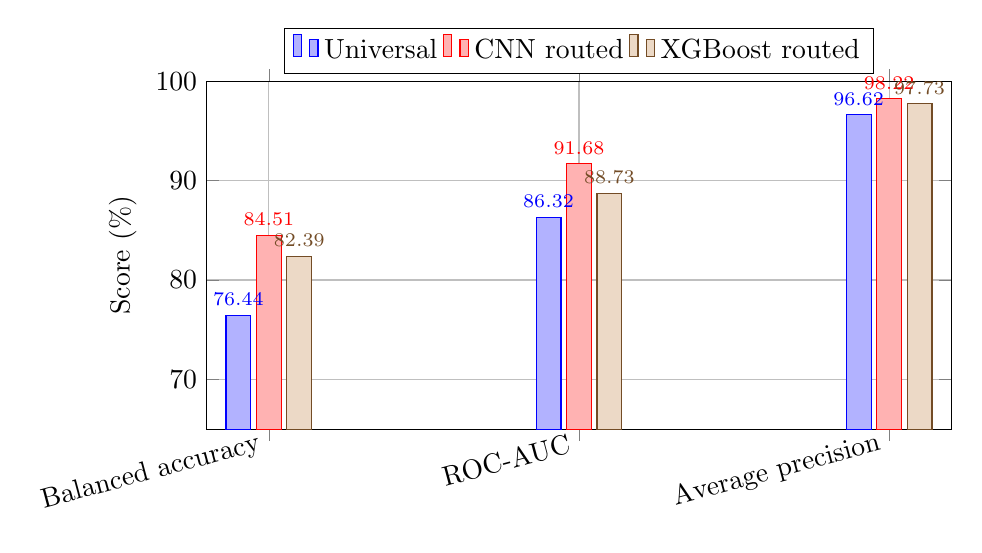
\begin{tikzpicture}
\begin{axis}[
  ybar, bar width=9pt, width=0.91\textwidth, height=60mm,
  ymin=65,ymax=100, ylabel={Score (\%)},
  symbolic x coords={Balanced accuracy,ROC-AUC,Average precision},
  xtick=data, x tick label style={rotate=15,anchor=east},
  legend style={at={(0.5,1.02)},anchor=south,legend columns=3},
  nodes near coords, nodes near coords style={font=\scriptsize},
  grid=major
]
\addplot coordinates {(Balanced accuracy,76.44) (ROC-AUC,86.32) (Average precision,96.62)};
\addplot coordinates {(Balanced accuracy,84.51) (ROC-AUC,91.68) (Average precision,98.22)};
\addplot coordinates {(Balanced accuracy,82.39) (ROC-AUC,88.73) (Average precision,97.73)};
\legend{Universal,CNN routed,XGBoost routed}
\end{axis}
\end{tikzpicture}
\caption{Aggregate routing comparison. The plot visualises the current six-way
artefact and must not be relabelled as the intended five-expert rerun.}
\label{fig:routing-bars}
\end{figure}

Per-method balanced accuracy in \Cref{tab:routing-method} explains why the idea
is promising. Every specialist outperforms the universal detector for its method,
and routing recovers part, but not all, of that oracle-like advantage. Router
mistakes therefore remain a measurable bottleneck. NeuralTextures is the hardest
of the five classes for the specialist and routed systems.

\begin{table}[H]
\centering
\setlength{\tabcolsep}{10pt}
\caption{Per-manipulation balanced accuracy of specialist, universal, and current
routed CNN systems (\%).}
\label{tab:routing-method}
\begin{tabular}{@{}lrrr@{}}
\toprule
Manipulation & Matched specialist & Universal & Routed CNN \\
\midrule
Deepfakes & 94.86 & 79.81 & 88.62 \\
Face2Face & 92.36 & 78.47 & 85.20 \\
FaceShifter & 93.24 & 75.70 & 87.64 \\
FaceSwap & 90.37 & 75.58 & 84.98 \\
NeuralTextures & 80.28 & 72.66 & 76.11 \\
\bottomrule
\end{tabular}
\end{table}

The result supports a narrow conclusion: under the saved group-disjoint,
in-domain FF++ protocol, method-conditioned specialist selection improves a
universal Xception baseline. It does not demonstrate robustness to unseen
generators, external datasets, recapture, injection, video-level aggregation, or
deployment demographics. It also incurs an expert-training and storage cost that
must be compared with stronger universal or multi-task baselines.

\subsection{Assessment against objectives}

\begin{table}[H]
\centering
\caption{Objective-level evaluation status.}
\label{tab:objective-status}
\begin{tabularx}{\textwidth}{@{}p{38mm}p{24mm}Y@{}}
\toprule
Objective & Status & Evidence-based assessment \\
\midrule
Mobile temporal prototype & Partial success & Integrated 24-frame local path;
checkpoint/training provenance and device profiling remain. \\
Temporal deepfake transfer & Investigated & $G^2V^2$former results expose severe
domain shift; not yet operationally adequate. \\
Domain-generalised comparison & Investigated & GD-FAS strong in-domain, limited
cross-domain; fine-tuning improves target but remains weak. \\
Specialist routing & Promising, incomplete & Current six-way routing outperforms
universal baseline; intended five-expert best-model formulation requires rerun. \\
Layered end-to-end system & Not completed & Mobile and API artefacts exist
separately; fusion, escalation, review, and IAD are target design. \\
Fairness, privacy, and security validation & Not completed & Risks and requirements are
documented; demographic, field, red-team, and governance evaluation remain. \\
\bottomrule
\end{tabularx}
\end{table}

\section{Deviations and Design Revisions}

The main deviations are substantive and should remain visible in the final report:

\begin{enumerate}
  \item The planned three-tier system was narrowed to an integrated mobile first
        stage and separately tested server candidates; no reviewer interface was
        completed.
  \item The temporal MobileNet training code uses 10-frame clips in one path,
        whereas export/inference/application code uses 24; the final artefact
        cannot inherit earlier metrics without provenance evidence.
  \item $G^2V^2$former checkpoint metrics differ between the latest PDF and saved
        artefacts and require one reproducible final evaluation.
  \item Strong physical-PAD performance did not transfer to digital deepfakes,
        motivating GD-FAS comparison and manipulation-specific Xception work.
  \item The routing notebook added an original class, although the intended
        meta-router only selects among five specialists. Its useful six-way result
        is reported honestly, and the corrected five-way experiment is future work.
  \item Capture-channel attacks became an explicit system concern. Media analysis
        alone is no longer represented as sufficient protection from injection.
\end{enumerate}

These revisions improve the report's validity: they separate demonstrated
evidence from architecture intent and convert unresolved contradictions into
testable follow-up work.

\chapter{Project Management, Teamwork, and Impact}
\label{ch:management}

\section{Project Management and Finance}

\subsection{Planning and Risk Management}

The work progressed from problem framing and a three-tier target architecture to
mobile temporal modelling, richer temporal analysis, domain-generalisation
comparison, integration, and finally specialist routing. \Cref{fig:timeline}
reconstructs this sequence in relative phases because verified calendar dates are
not yet consolidated. It must be replaced by the actual baseline and completion
dates before submission.

\begin{figure}[H]
\centering
\begin{ganttchart}[
  hgrid,vgrid,
  x unit=15mm,
  y unit chart=6mm,
  title label font=\small\bfseries,
  bar label font=\scriptsize,
  bar/.append style={fill=buetblue!65}
]{1}{8}
\gantttitle{Relative project phase}{8}\\
\gantttitlelist{1,...,8}{1}\\
\ganttbar{Proposal and requirements}{1}{1}\\
\ganttbar{Architecture and threat model}{1}{2}\\
\ganttbar{MobileNet and Flutter}{2}{5}\\
\ganttbar{$G^2V^2$former experiments}{3}{5}\\
\ganttbar{GD-FAS and data preparation}{5}{6}\\
\ganttbar{Mobile/API integration work}{5}{7}\\
\ganttbar{Xception specialists/routing}{7}{8}\\
\ganttbar{Synthesis and final report}{8}{8}
\end{ganttchart}
\caption{Draft reconstruction of project progression. Phase indices show order
and overlap, not verified calendar dates.}
\label{fig:timeline}
\end{figure}

\begin{longtable}{@{}p{35mm}p{42mm}p{55mm}@{}}
\caption{Principal project risks and mitigations.}\label{tab:risks}\\
\toprule
Risk & Consequence & Mitigation and remaining action \\
\midrule
\endfirsthead
\toprule
Risk & Consequence & Mitigation and remaining action \\
\midrule
\endhead
Frame/identity leakage & Inflated validation performance & Split by source-video
group; audit every dataset at identity and derivation level. \\
Domain or generator shift & Failure on new attacks despite high source accuracy &
Cross-dataset evaluation, diverse training, unseen-generator holdout, drift
monitoring, conservative escalation. \\
Class imbalance & Misleading accuracy and unsafe threshold & Report balanced
accuracy and class rates; calibrate on deployment prevalence/cost. \\
Router failure & Correct expert is bypassed & Report oracle/specialist gaps,
top-$k$ or soft-routing ablations, and a safe universal fallback. \\
Capture injection & Classifier receives convincing forged media & Device/sensor
attestation, protected channel, replay defence, IAD and red-team testing. \\
Biometric disclosure & Irreversible privacy harm & Minimise collection, encrypt,
separate identifiers, restrict access, delete by policy, incident response. \\
False rejection & Exclusion and repeated exposure & Accessible recapture, bounded
retry, alternative verification, timely appeal and review. \\
Training instability or missing checkpoint & Irreproducible claims & Freeze
environment/configuration/checksum and regenerate result tables from artefacts. \\
Model obsolescence & New manipulations evade detection & Versioned monitoring,
red-team sets, retraining triggers, rollback, and maintained ownership. \\
Scope inflation & Prototype presented as product & Maintain implemented,
experimental, and proposed labels in architecture and claims. \\
\bottomrule
\end{longtable}

\subsection{Budgeting and Resource Identification}

An earlier weekly report planned a USD 260--540 GPU budget. That range is a plan,
not evidence of expenditure. The final cost record must distinguish free notebook
quotas, personally owned devices, any paid compute/storage, internet use, and
personnel time.

\begin{table}[H]
\centering
\caption{Draft resource and budget record.}
\label{tab:budget}
\begin{tabularx}{\textwidth}{@{}p{39mm}p{33mm}Y@{}}
\toprule
Resource & Recorded cost & Evidence/status \\
\midrule
GPU compute & Planned USD 260--540 & Earlier estimate only; actual provider,
hours, tier, and payment \TBC{actual compute record}. \\
Local development devices & \TBC{cost basis} & Personally owned laptops/phones;
record models and whether an incremental project cost was incurred. \\
Storage and network & \TBC{actual cost} & Public dataset transfer and artefact
storage; record paid services and retention. \\
Software & USD 0 licence cost for main tools & Primarily open-source research and
development stack; licence obligations still apply. \\
Human effort & \TBC{person-hours} & Student effort should be reported separately
from cash spending; production review would be a recurring cost. \\
Partner/dataset grant & USD 0 received & No project grant or private dataset was
provided by Pathao or a dataset owner. \\
\bottomrule
\end{tabularx}
\end{table}

\subsection{Economic Analysis and Financial Prospecting}

The cascade is economically attractive only if local screening reduces server
and review cost without increasing fraud or abandonment beyond acceptable limits.
For $N$ sessions, a transparent expected-cost model is
\begin{equation}
C=N(C_{\mathrm{edge}}+r_sC_{\mathrm{server}}+r_hC_{\mathrm{review}})
 + N_{\mathrm{FA}}L_{\mathrm{fraud}}
 + N_{\mathrm{FR}}L_{\mathrm{friction}},
\end{equation}
where $r_s$ and $r_h$ are escalation and review rates. The loss terms must be
estimated from partner evidence rather than borrowed percentages. Calibration
curves can then show how changing a threshold moves cost between compute, review,
false acceptance, and false rejection.

No financial return is claimed in this project because production prevalence,
fraud loss, abandonment, reviewer cost, and integration cost were not supplied.
The useful output is the model above and the measurements needed to populate it.

\subsection{Sustainability in Business and Commercialisation}

A responsible path is: reproducible research validation; licence/privacy/security
review; partner-specific data collection with consent; red-team and independent
PAD/IAD evaluation; monitored shadow deployment; a limited pilot with appeal; and
only then a staged rollout. Long-term ownership must cover model monitoring,
incident response, reviewer training, data retention, accessibility, compliance,
and retirement of obsolete models. A specialist bank increases maintenance cost;
its gain must persist against a stronger universal model before commercial use.

\section{Individual and Teamwork}

\subsection{Participation and Contribution}

The candidate list is established, but the repository alone cannot determine all
research, presentation, debugging, coordination, and writing effort. The team
must validate \Cref{tab:contributions} jointly against notebooks, commits,
reports, slides, and meeting records rather than treating an early assigned role
as an achieved contribution.

\begin{table}[H]
\centering
\caption{Contribution record to be verified by the team.}
\label{tab:contributions}
\begin{tabularx}{\textwidth}{@{}p{43mm}p{24mm}Y@{}}
\toprule
Candidate & Student ID & Verified concrete contributions and delivery evidence \\
\midrule
Nafis Nahian & 2105007 & \TBC{implementation, experiments, reports,
integration, review, coordination, and deadlines}. \\
Abrar Zahin Raihan & 2105009 & \TBC{implementation, experiments, reports,
integration, review, coordination, and deadlines}. \\
Aritra Debnath & 2105010 & \TBC{implementation, experiments, reports,
integration, review, coordination, and deadlines}. \\
Tamzeed Mahfuz & 2105012 & \TBC{implementation, experiments, reports,
integration, review, coordination, and deadlines}. \\
Ruwad Naswan & 2105051 & \TBC{implementation, experiments, reports,
integration, review, coordination, and deadlines}. \\
\bottomrule
\end{tabularx}
\end{table}

\subsection{Collaboration and Conflict Resolution}

The project required agreement on dataset protocols, checkpoint selection,
metric definitions, integration contracts, and how to interpret negative results.
A reproducible collaboration process uses issue-level ownership, peer review,
shared experiment manifests, named decision records, and explicit escalation when
results conflict. The unresolved 10/24-frame and HTER discrepancies demonstrate
why numerical disagreements must be resolved through artefacts and reruns rather
than preference. \TBC{Add one or two verified examples of a disagreement, the
alternatives considered, the resolution, and its effect on schedule or design.}

\subsection{Leadership and Direction}

Technical leadership in this project includes narrowing claims after cross-domain
failure, assigning reproducibility work, protecting time for integration, and
raising privacy/security issues before deployment. The supervisor provided major
research direction and originated the specialist-routing idea. \TBC{Identify the
student leads for each phase and document how they delegated, reviewed work, and
handled missed milestones.}

\subsection{Multidisciplinary Engagement}

The work combines machine learning, mobile software, backend deployment,
cyber-security, human--computer interaction, financial risk, biometric privacy,
and professional ethics. A production team would additionally require fraud
operations, accessibility, legal/compliance, incident response, and customer
support. The engineering decision is not solely which classifier has the largest
AUC: it includes capture provenance, consent, threshold costs, user recourse,
reviewer workload, and maintainability.

\section{Impact on Society}

Reliable remote verification can widen access, reduce impersonation, and allow a
customer to complete a sensitive process without travel. The same system can
also deny service, intensify surveillance, or expose biometric data. Impact is
therefore conditional on who can use the capture flow, whose faces and devices
were represented during evaluation, what happens after rejection, and whether a
customer can challenge a decision.

False acceptance may harm the impersonated person and the provider. False
rejection may disproportionately burden people with older cameras, unstable
connectivity, darker or lighter skin under poor illumination, facial differences,
religious attire, disability, or difficulty performing an active challenge.
Repeated retry can itself increase biometric exposure and frustration. Socially
responsible deployment requires an equivalent alternative verification route,
clear notice, bounded retry, timely human appeal, accessible instructions, and
regular publication of aggregate error and override behaviour where safe.

\section{Environmental Impact and Life Cycle Sustainability}

GPU training, repeated hyperparameter search, dataset replication, network
transfer, server escalation, and retained video all consume energy and storage.
The cascade may reduce serving energy by resolving clear cases locally, but mobile
battery use and the embodied impact of devices still matter. A five-expert bank
also multiplies training and storage unless sharing or distillation is used.

The environmental plan is to record GPU type and hours; reuse frozen embeddings
for router ablations; stop unpromising runs early under a declared rule; cache
preprocessing safely; select the smallest model meeting validated requirements;
limit media retention and duplication; batch server work where latency allows;
and measure energy/latency per accepted, escalated, and reviewed transaction.
Lifecycle planning must include model replacement and secure deletion, not only
initial training.

\section{Ethics}

Ethical analysis is a design constraint throughout the pipeline. The main risks,
controls, and missing evidence are shown in \Cref{tab:ethics}.

\begin{longtable}{@{}p{31mm}p{52mm}p{50mm}@{}}
\caption{Ethical risk--control--evidence matrix.}\label{tab:ethics}\\
\toprule
Risk & Required control & Evidence still required \\
\midrule
\endfirsthead
\toprule
Risk & Required control & Evidence still required \\
\midrule
\endhead
Biometric privacy & Purpose limitation, minimisation, encryption, separated
identifiers, least privilege, deletion, breach process & Data inventory, retention
schedule, access audit, deletion test, incident exercise \\
Inadequate consent & Plain-language notice of purpose, processing, retention,
sharing, alternatives, and appeal & Comprehension/usability study and approved
notice \\
Demographic disparity & Representative evaluation, subgroup error/calibration,
intersectional testing, mitigation and stop criteria & Consented demographic
protocol and sufficiently powered results \\
Device/network disparity & Quality-aware capture, low-bandwidth behaviour,
supported-device testing, alternative path & Device matrix and field trials \\
False rejection & Bounded retry, accessible recapture, reason categories,
alternative verification and human appeal & FRR by condition/group; appeal time,
overturn and abandonment rates \\
False acceptance & Capture integrity, PAD/IAD, red-team tests, conservative high-
risk policy and monitoring & Attack-presentation and injection test campaign \\
Selective escalation bias & Audit who is escalated/reviewed and outcome gaps;
calibrate by policy without discriminatory shortcuts & Escalation, review, and
override rates by relevant subgroup and device condition \\
Reviewer automation bias & Show uncertainty/evidence limits, train reviewers,
blind irrelevant attributes, sample QA and second review & Human-factors study and
inter-reviewer consistency \\
Dual-use disclosure & Publish enough for reproducibility while withholding
operational secrets that materially ease bypass; responsible vulnerability route &
Threat-informed release and disclosure plan \\
Dataset/IP misuse & Licence/provenance audit, minimum redistribution, attribution,
and removal process & Dataset-by-dataset permission record \\
\bottomrule
\end{longtable}

\subsection{Equity and Inclusivity}

Aggregate AUC can conceal unequal false-accept and false-reject rates. Evaluation
should pre-register relevant groups and capture conditions, avoid using sensitive
attributes as unexplained proxies, report uncertainty, and investigate
intersections where sample size permits. Asian-Fakes provides one additional
domain but is not, by itself, proof of demographic fairness. A face dataset's name
or geographic origin does not guarantee a balanced or consented fairness sample.

The user interface should not require speech, hearing, a narrow range of facial
motion, expensive hardware, or sustained high bandwidth without an equivalent
alternative. Escalation and review are also fairness surfaces: a group sent to
review more often experiences delay and greater human scrutiny even if the final
acceptance rate appears equal.

\subsection{Accountability and Personal Responsibility}

Every decision should be attributable to a model version, configuration,
threshold policy, quality state, and responsible owner. Model developers are
responsible for reporting limitations; product owners for appropriate use;
security teams for capture/channel controls; reviewers for reasoned decisions;
and management for resourcing appeal and incident response. A human reviewer must
not become an accountability sink: override rules, evidence access, second review,
quality sampling, and appeal outcomes require governance.

The candidates accept responsibility for distinguishing completed work from
proposal, retaining contradictory results until reconciled, and correcting the
routing formulation. High performance on one benchmark must never be advertised
as comprehensive fraud prevention.

\subsection{Proper Use of Intellectual Property}

\begin{table}[H]
\centering
\caption{Third-party asset and attribution inventory.}
\label{tab:ip}
\begin{tabularx}{\textwidth}{@{}p{34mm}Y Y@{}}
\toprule
Asset & Use & Required action \\
\midrule
FaceForensics++, Celeb-DF-v2, LCC-FASD, Asian-Fakes, ROSE-Youtu & Research data &
Verify access terms, citation, redistribution, consent/provenance, and derivative
frame policy separately. \\
$G^2V^2$former and GD-FAS & Adapted research methods/code & Cite papers and
repositories; preserve licence notices; document modifications and weights. \\
MobileNetV3 and Xception & Model architectures/pretrained components & Cite
original work; record library/weight licence and version. \\
PyTorch, Flutter, FastAPI, XGBoost and supporting libraries & Implementation stack &
Maintain dependency bill of materials and comply with their licences. \\
BUET logo and report template & Institutional report material & Use only for the
course report and preserve required formatting/attribution. \\
Generative-AI assistance & Drafting/editing support & Disclose per course policy;
students verify all content and do not assign authorship to the tool. \\
\bottomrule
\end{tabularx}
\end{table}

No dataset, code, or figure should be redistributed merely because it is publicly
accessible. The final repository release should include only artefacts allowed by
their licences and access agreements.

\subsection{Professionalism and Ethical Codes}

The ACM and IEEE codes emphasise avoiding harm, honesty about system limitations,
respect for privacy, fairness, competence, and responsibility
\cite{acmcode,ieeecode}. Applied here, professionalism means resisting pressure
to turn benchmark numbers into deployment guarantees; documenting negative and
contradictory results; protecting captured faces; obtaining expertise outside
machine learning; and suspending or rolling back a system when monitored harm
exceeds agreed thresholds. Security details should be disclosed responsibly, and
affected users should receive meaningful explanation and recourse.


\chapter{Conclusion}
\label{ch:conclusion}

\section{Conclusion and Future Work}

This capstone investigated liveness verification as a layered engineering problem,
not as a single binary-classification benchmark. The implemented work spans a
lightweight temporal MobileNetV3 mobile path, explicit temporal modelling with
$G^2V^2$former, domain-generalised spatial analysis with GD-FAS, public-data
preparation and transfer experiments, a separate server prototype, and later
manipulation-specific Xception routing. Together these components reveal both the
promise and the current limits of robust remote face verification.

The objectives were met unevenly but informatively. A 24-frame local inference
flow is integrated in Flutter, although its checkpoint provenance and device
performance need a final audit. $G^2V^2$former and GD-FAS were evaluated across
physical-PAD and deepfake domains. Their results show that excellent source-domain
performance can collapse under a change in attack family, and that target-domain
fine-tuning improves some results without solving unseen-domain generalisation.
The later FF++ experiment shows that matched specialists and learned routing can
improve an in-domain universal Xception baseline: the current CNN-routed artefact
raises balanced accuracy from 76.44\% to 84.51\% and ROC-AUC from 86.32\% to
91.68\%. That finding is promising but narrow, because the saved router includes
an original class and has not been tested against unseen generators, injection,
or deployment populations.

The strongest project conclusion is therefore methodological. Physical
presentation attacks, digital manipulation, and capture-channel injection require
different but coordinated evidence. Temporal reasoning can contribute, domain
generalisation must be measured rather than assumed, and manipulation specialists
may help when their routing targets and evaluation are leakage-safe. None of
these replaces genuine-sensor assurance, protected transport, calibrated policy,
privacy protection, subgroup evaluation, or accountable recourse.

The next work should proceed in the following order:

\begin{enumerate}
  \item freeze an experiment manifest and reconcile the MobileNetV3 sequence
        length/checkpoint and $G^2V^2$former metric discrepancies;
  \item rebuild the router as a five-expert selector with no original class,
        using out-of-fold expert predictions if the target is ``best expert'';
  \item compare method-label routing, true best-expert routing, oracle routing,
        top-$k$/soft routing, and a stronger universal or multi-task baseline;
  \item evaluate all deepfake systems at video level on unseen generators,
        additional compression/recapture, and independent external datasets;
  \item calibrate scores and produce reliability, threshold-cost, and escalation-
        coverage curves rather than adopting a universal 0.5 threshold;
  \item connect the mobile and server components through an authenticated,
        versioned contract and implement failure-safe offline/network behaviour;
  \item add genuine-camera confidence, replay protection, device integrity, and
        injection red-team scenarios rather than relying on media analysis alone;
  \item conduct representative device, demographic, accessibility, privacy, and
        reviewer studies with explicit stop criteria and appeal measurement; and
  \item evaluate latency, memory, bandwidth, energy, serving/review cost, licence
        compliance, monitoring, rollback, and secure deletion in a governed pilot.
\end{enumerate}

A human-review path should be implemented only with trained reviewers, bounded
evidence access, reason codes, second-review rules, workload testing, and user
appeal. It should not be described as a generic cure for model uncertainty.

\section{Continuous Engagement and Self-directed Learning}

The project required continuous learning across research and engineering
boundaries. The team moved from an initial mobile/server concept to video
transformers and landmark motion, then to domain-generalisation methods, mobile
model export, API prototyping, Xception specialists, and routing ablations. Reading
primary papers was necessary but insufficient: implementations had to be adapted,
dataset structures reconciled, numerical issues debugged, checkpoints interpreted,
and results compared under common metrics.

Negative transfer results were particularly valuable. They changed the project
from a search for one high score into an investigation of attack taxonomy,
dataset shift, and evidence boundaries. The injection threat similarly expanded
the design beyond classifier accuracy to capture provenance and channel security.
The routing discrepancy reinforced a further lesson: a mathematically attractive
claim is valid only when labels, data splits, code paths, and evaluation actually
implement it.

Professional development should continue through reproducible experiment
packaging, biometric security and privacy study, mobile profiling, secure
deployment, calibration, human-factors evaluation, and responsible disclosure.
Future engagement with a financial partner should begin with jointly defined
threats, lawful and consented data governance, operational error costs, and pilot
stop conditions. These practices are as important to trustworthy liveness
verification as further model optimisation.



\clearpage
\bibliographystyle{IEEEtran}
\bibliography{references}

\appendix
\chapter{Draft Verification Checklist}
\label{app:checklist}
The following items must be resolved against primary records before the report is
submitted: supervisor identity and title; academic session and submission date;
the team contribution record; actual expenditure; dataset licence statements;
the MobileNetV3 training--export sequence-length mismatch; G2V2Former checkpoint
and metric reconciliation; and rerunning the router with the intended five-expert,
no-original target. All statements concerning an unintegrated server, fusion,
human review, capture attestation, or injection defence must remain labelled as
proposed until an end-to-end artefact and evaluation exist.

\end{document}

